\scanpage{165}

\begin{flushleft}
U N I V E R S I T E\\
DES SCIENCES ET TECHNIQUES\\
DU LANGUEDOC\\
------------\\
Service de la Scolarité\\
MA/IE\\
\uline{Diffusion} : liste A\\
n°4584
\end{flushleft}
\begin{flushright}MONTPELLIER, le 16 septembre 1980\end{flushright}

\begin{center}
\uline{AVIS DE SOUTENANCE D'UNE THESE DE DOCTORAT DE 3ème CYCLE} :

\uline{AGRONOMIE Option ZOOTECHNIE}
\end{center}

\uline{Nom et prénom du candidat} : PEREZ MURUA Oscar

\uline{Titre de la thèse} : Influence du mode de conduite sur le comportement maternel et quelques paramètres zootechniques chez la vache Française Frisonne Pie Noire (FFPN) en lactation.

\uline{Date, heure et lieu de soutenance prévus} : 26 septembre 1980 à 14 H 30 au laboratoire de Zootechnie - ENSAM, Montpellier

\uline{Nom du Directeur de la thèse} : Monsieur le Professeur DAUZIER

\uline{Désignation du laboratoire où la thèse est préparée} : laboratoire de Physiologie de la Reproduction, INRA Nouzilly

\uline{Analyse de l'ouvrage} : Nous avons étudié le comportement maternel des vaches soumises à 3 modes de conduite : allaitement libre de 3 veaux par vache après une période d'adoption, allaitement surveillé de 3 veaux par vache deux fois par jour et traite deux fois par jour.

Nous avons trouvé une influence sur le comportement maternel, la production laitière et le taux de prolactine dans le sang lors de la stimulation mammaire selon le mode de conduite des vaches. Egalement, la croissance des veaux a été affectée par la qualité de l'adoption.

\uline{Durée approximative des recherches ayant abouti à la thèse} : 3 ans.

\uline{Composition du jury proposé} : MM. : \begin{tabular}[t]{l}
DAUZIER\\
SIGNORET\\
LEGRAND\\
PRUD'HON
\end{tabular}

\begin{flushright}
P/le Secrétaire Général\\
L'Attachée d'Administration Universitaire,

\figure{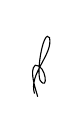
\begin{tikzpicture}[x=1cm,y=1cm]
\draw (0,0) .. controls (-.08,.25) and (.24,.5) .. (.19,.71) .. controls (.12,.83) and (.02,.31) .. (.07,.17) .. controls (.18,.01) and (.15,.37) .. (.01,.36) .. controls (-.08,.3) and (.03,.01) .. (.04,-.04);
\end{tikzpicture}}
\uline{\unsure{Gentil}}\\
\uline{A. GENTIL}
\end{flushright}

\margin{165}
